\documentclass[12pt]{report}
\PassOptionsToPackage{sharp}{prettytex/boxes}
\usepackage{prettytex/base}
\usepackage{prettytex/math}
\usepackage{prettytex/math-theorems}
\usepackage{prettytex/gfx}
\usepackage{prettytex/code}
\usepackage{prettytex/thesis}
\usepackage[bsc,claim,iaik]{iaikthesis}
\usepackage{tabularray}
\usepackage{neuralnetwork}

\thesistitle{
  Secure Classification as a Service \\
  \small\normalfont Levelled Homomorphic, Post-Quantum Secure Machine Learning Inference \\
  based on the CKKS Encryption Scheme
}
\thesisauthor{Peter Julius Waldert}
\thesisdate{March 2022}
% \thesistitleimage{}
\supervisortitle{Supervisors}
\supervisor{
  Dipl.-Ing. Roman Walch \\
  \vspace{0.4cm}
  \href{https://www.iaik.tugraz.at/}{\textcolor{black}
    {Institute of Applied Information Processing and Communications (IAIK)}} \\
  \href{https://www.tugraz.at/}{\textcolor{black}
    {Graz University of Technology}}
}
\curriculum{\textit{Physics} and \textit{Information \& Computer Engineering}}

\title{\@thesistitle}
\author{\@thesisauthor}

\setlength{\headheight}{19.53pt}

\makenoidxglossaries
\newacronym{he}{HE}{Homomorphic Encryption}
\newacronym{fhe}{FHE}{Fully Homomorphic Encryption}
\newacronym{bfv}{BFV}{Brakerski-Fan-Vercauteren}
\newacronym{bgv}{BGV}{Brakerski-Gentry-Vaikuntanathan}
\newacronym{ckks}{CKKS}{Cheon-Kim-Kim-Song}
\newacronym{rsa}{RSA}{Rivest-Shamir-Adleman}
\newacronym{aes}{AES}{Advanced Encryption Standard}
\newacronym{lwe}{LWE}{Learning With Errors}
\newacronym{dlwe}{DLWE}{Decision Learning With Errors}
\newacronym{rlwe}{RLWE}{Learning With Errors on Rings}
\newacronym{tls}{TLS}{Transport Layer Security}
\newacronym{ml}{ML}{Machine Learning}
\newacronym{gd}{GD}{Gradient Descent}
\newacronym{mse}{MSE}{Mean-Squared-Error}
\newacronym{dft}{DFT}{Discrete Fourier Transform}
\newacronym{fft}{FFT}{Fast Fourier Transform}
\newacronym{iff}{iff}{if and only if}
\newacronym{np}{NP}{Non-deterministic Polynomial time}
\newacronym{ppml}{PPML}{Privacy-Preserving Machine Learning}
\newacronym{mnist}{MNIST}{Modified National Institute of Standards and Technology database}
\newacronym{sis}{SIS}{Shortest Integer Solution}
\newacronym{svp}{SVP}{Shortest Vector Problem}
\newacronym{gapsvp}{GapSVP}{Decisional Approximate Shortest Vector Problem}
\newacronym{fhew}{FHEW}{Fastest Homomorphic Encryption in the West}
\newacronym{tfhe}{TFHE}{Torus Fully Homomorphic Encryption}
\newacronym{crt}{CRT}{Chinese Remainder Theorem}
\newacronym{rns}{RNS}{Residue Number System}

\newcommand{\cpp}[1]{\mintinline{cpp}{#1}}
\newcommand{\name}[1]{\textsc{#1}}
\newcommand{\cryptop}[1]{\text{\textcolor{darkpurple}{#1}}}
\newcommand{\inv}{^{-1}}
\newcommand{\inputtikz}[1]{
  % \tikzsetnextfilename{#1}
  % \input{#1.tex}
  \vspace{2cm}
  Placeholder
  \vspace{2cm}
}

\addbibresource{sources.bib}

\begin{document}
  \printthesistitle
  \chapter*{Abstract}
The rapid developments in quantum computation affect cryptography as it is used today.
With a sufficiently powerful quantum computer, most digital communication could be decrypted in polynomial time by an eavesdropping party with access to such a potent utility, posing a major problem to the worldwide community.
Lattice-based cryptographic schemes aim to mitigate this, while including many further advantages, which will be the main topic of this thesis.

With technological advancements in machine learning, problems long thought to be impossible can now be solved by complicated and resource-intensive neural network structures.
Machine learning undoubtedly holds many new possibilities, especially in medicine, although large datasets are scarce in this area.
\Gls{ppml} is an emerging field in data science that focusses on leveraging such highly private data anyway, without ever actually seeing it.
The techniques behind this are homomorphic encryption schemes, two of which this thesis will discuss in detail.
% Using fully homomorphic encryption schemes, an encrypted dataset can be operated on without ever having the possibility to decrypt it, not even with a quantum computer.

To demonstrate the possibilities of these homomorphic cryptosystems applied to machine learning inference, a web-based demonstrator was developed (confer \cref{fig:frontend}).
The backend server is written in C++, using the Microsoft \glstext{seal} homomorphic encryption library.
This work starts by introducing the necessary mathematical background, motivating the definitions of the \glstext{bfv} and \glstext{ckks} encryption schemes in the following chapter and describing the basics of machine learning along the way.
The principles and implications of \name{Shor}'s algorithm are discussed, further inciting the need for studying the hardness of the \glstext{lwe}-based cryptosystems.
The final chapters then focus on implementation aspects, the analysis of obtained results and performance benchmarks.

\paragraph{Keywords:}
FHE, ML, Image Classification, Neural Network,
Private AI, PPML, Confidential Computing,
Post-Quantum Security

\paragraph{Technologies:}
Microsoft SEAL (C++, NodeJS),
Tensorflow Keras,
Numpy,
xtensor,
Docker,
msgpack,
React,
Materialize,
Nginx

\paragraph{Languages:}
C++, Python, JavaScript

  \tableofcontents
  \chapter{Introduction}
\label{chap:introduction}
The most well-known and widely used asymmetric ('public-key') cryptographic scheme, published by the trio \name{Rivest}-\name{Shamir}-\name{Adleman} in 1977 and known as \textit{RSA}, is based on the hardness assumption of the integer factorisation problem (factorising a large 2-composite number into its two prime factors $p$ and $q$ is hard).
As of today, this factorisation problem has not been proven to be in NP, yet it is suspected that it might indeed be NP-complete (i.e. \hyperref[def:np-hard]{NP-hard} while still being in NP) when modelled using a traditional Turing machine.
Since the advent of quantum computation, this situation changed as a whole with Peter \name{Shor}'s algorithm, threatening the security of many cryptosystems, for instance RSA which is still widely used today despite its known problems.

As it stands, lattice-based cryptography presents a solution to a politically and socially problematic situation in which few parties world-wide, with access to a sufficiently powerful quantum computer, may be able to decrypt most of today's digital communication.
\hyperref[subsec:lattice-crypto]{Lattice Cryptography} is based on other mathematical problems, shown to be sufficiently hard on quantum computers and traditional ones alike, most notably \hyperref[def:lwe-search-problem]{LWE} which this thesis will discuss in detail.

Many new cryptosystems have been developed on top of LWE, two of which this following thesis will focus on specifically: \hyperref[def:bfv-scheme]{BFV} and \hyperref[def:ckks-scheme]{CKKS};
whose security is still unaffected by efficient quantum algorithms.
Yet, it is not only their security prospect that makes these encryption schemes attractive, but first and foremost their defining \hyperref[def:ring-homomorphism]{homomorphic} property which allows for computations on the encrypted data.
A \textit{fully} homomorphic encryption (FHE) scheme was first introduced by Craig \name{Gentry} in 2009, using a bootstrapping approach.
The \textit{levelled} homomorphic \gls{bgv} encryption scheme is implemented in Microsoft SEAL and allows for integer arithmetic, up to a few multiplication 'levels' deep.
The \gls{bfv} scheme is very similar to it and described in a bit more detail in \autoref{sec:bfv}.
And finally, building upon concepts introduced in the former, the \gls{ckks} scheme allows for approximative floating-point arithmetic that finally facilitates machine-learning applications.

Machine Learning allows a computer to 'learn' from specifically structured data using linear regression or similar methods, and applying this 'knowledge' to new, unknown inputs.
In its simplest form, or even using a neural network, this only requires two different operations on numbers (or even better, vectors): addition and multiplication.
Using an \gls{he} scheme such as the ones mentioned above and described in \autoref{chap:homomorphic-encryption}, both are given and PPML (Privacy-Preserving Machine Learning) applications are born!

Considering the implications of mass surveilance, the importance of privacy-preserving/enhancing technologies should not be forgotten.

The present thesis not only focusses on theoretical remarks but also includes a publicly available implementation of an \gls{he} classification server written in C++ and a compact graphical user interface to interact with.
The following aims to introduce most of the necessary theory to understand the homomorphic encryption schemes used in practice today, as well as the simple machine learning approaches involved in securely classifying images as a service.

  \chapter{Background}
\label{chap:background}

\section{Basics of Fully Homomorphic Encryption}
\gls{he} makes it possible to operate on data without knowing it.
One can distinguish three flavors of it, Partial-, Somewhat- and \gls{fhe}.

For \Gls{fhe}, there exist a few schemes in use today with existing implementations.
\begin{itemize}
  \item Brakerski/Fan-Vercauteren (BFV) scheme for integer arithmetic
        (\cite{2012-fv-original}, \cite{2012-brakerski}).
  \item Brakerski-Gentry-Vaikuntanathan (BGV) scheme for integer arithmetic \parencite{2012-bgv-original}.
  \item Cheon-Kim-Kim-Song (CKKS) scheme for real-number arithmetic \parencite{2017-ckks-original}.
  \item Ducas-Micciancio (FHEW) and Chillotti-Gama-Georgieva-Izabachene (TFHE) schemes for Boolean circuit evaluation
        \parencite{2019-tfhe-original}.
\end{itemize}

We will first introduce the BFV scheme (integer arithmetic) as it represents a fundamental building block behind CKKS.
Due to the inherent applications, this thesis will focus on the CKKS scheme to perform homomorphic operations
on (complex-valued) floating point numbers and vectors.

\subsection{Mathematical Foundation}
The following discussion of the homomorphic encryption schemes requires some mathematical background that
will (at least partially) be introduced here.

\begin{definition}{Ring}{ring}
  A tuple $(R, +, \cdot)$ consisting of a set $R$, an addition operation $+$ and a multiplication operation $\cdot$
  is referred to as a ring, given that it satisfies the following \textit{ring axioms}:
  \begin{itemize}
    \item Addition is closed: $a + b \in R \quad\forall a, b \in R$.
    \item Addition is commutative: $a + b = b + a \quad\forall a, b \in R$.
    \item Addition is associative: $(a + b) + c = a + (b + c) \quad\forall a, b, c \in R$.
    \item There exists an element $0 \in R$ such that $a + 0 = a \quad\forall a \in R$.
    \item An additive inverse $-a$ of each element $a$ in $R$ exists, such that $a + (-a) = 0$.
    \item Multiplication is associative: $(a \cdot b) \cdot c = a \cdot (b \cdot c) \quad\forall a, b, c \in R$.
    \item Multiplication is closed: $a \cdot b \in R \quad\forall a, b \in R$.
    \item There exists an element $1 \in R$, referred to as the identity element, or multiplicative identity of $R$,
          such that $a \cdot 1 = a \quad\forall a \in R$.
    \item Multiplication $\cdot$ is distributive w.r.t. addition $+$, \\
          i.e. $a \cdot (b+c) = (a \cdot b) + (a \cdot c) \quad\forall a, b, c \in R$ from the left and \\
          i.e. $(b+c) \cdot a = (b \cdot a) + (c \cdot a) \quad\forall a, b, c \in R$ from the right.
  \end{itemize}
  Where the first 5 properties can be summarised as $(R, +)$ forming an Abelian group.
  If multiplication is additionally commutative, we refer to the ring as commutative:
  \begin{itemize}
    \item Multiplication is commutative: $a \cdot b = b \cdot a \quad\forall a, b \in R$.
  \end{itemize}
\end{definition}
Acting as a logical extension of a group, a ring can be considered the intermediary step towards a field
(which also defines subtraction and division).
An example of a ring would be the integers modulo $t$: $\Z / t \Z$, sometimes also denoted as $\Z_t$.

\begin{definition}{Quotient Group / Ring}{quotient-group}
  A quotient group $(G / N, +)$ (pronounced '$G$ mod $N$') over the original group $G$ and a normal subgroup $N$ of $G$
  with a standard element operation $+$ can be defined using the
\end{definition}

\begin{definition}{Ring of Integers Modulo $t$: $\Z / t \Z$}{integers-modulo-t}
  Using equivalence classes $\overline{x}_t$ modulo $t$ referred to as congruence classes,
  define the commutative quotient ring of integers modulo $t$ as
  $$\Z / t \Z = \{\overline{x}_t \,|\, x \in \Z, 0 \leq x < t\}$$
  where $t \Z \triangleleft \Z$ denotes the $t$\textsuperscript{th} coset\footnote{
    from the left and from the right, therefore $t \Z$ is called a normal subgroup of $\Z$
  } of the integers and
  $$\overline{x}_t = \{y \equiv x \mod t \,|\, y \in \Z\}$$
  is the set of all multiples of $t$ with remainder $x$.
\end{definition}

\begin{definition}{Polynomial Ring over $\Z$}{poly-ring}
  On the set of all complex-valued polynomials with integer coefficients (a function space)
  $$\Z[X] = \big\{p: \C \mapsto \C \,, p(X) = \sum_{k=0}^\infty a_k X^k, a_k \in \Z \;\forall k \geq 0\big\},$$
  we can define a commutative ring $(\Z[X], +, \cdot)$ equipped with the
  standard addition $+$ and multiplication $\cdot$ operations (as an extension over the field $\C$)
  of polynomials.
\end{definition}

% TODO: make p, q sequences instead of vectors
To further elaborate on the polynomial ring operations:
\begin{itemize}
  \item In their coefficient representations $(\vec{p})_i = p_0, p_1, p_2, ...$ (which are sequences) and $\vec{q} = \{q_0, q_1, q_2, ...\}$,
        an addition of two polynomials $p, q \in \Z[X]$ is equivalent to the addition of their coefficients
        \begin{align*}
          (p + q)(X) & = \sum_{k=0}^\infty p_k X^k + \sum_{k=0}^\infty q_k X^k = \sum_{k=0}^\infty (p_k + q_k) X^k \\
                     & = \langle (\vec{p} + \vec{q}), \{X^0, X^1, X^2, ...\}^T \rangle
        \end{align*}
        which indeed satisfies the additive \hyperref[def:ring]{ring axioms}
        due to the existing structure of the underlying field $\C$.
  \item The multiplication operation can be defined using a discrete convolution of the coefficient vectors
        $$r(X) = (p \cdot q)(X) = (\sum_{k=0}^\infty p_k X^k) \cdot (\sum_{l=0}^\infty q_l X^l)
          = \sum_{k=0}^\infty \sum_{l=0}^\infty p_k q_l X^{k+l}
          = \sum_{k=0}^\infty r_k X^k$$
        with the arising coefficients $\{r_k\}$ determined by the discrete convolution
        $$r_k = \sum_{l=0}^k p_l q_{k-l} \;\Leftrightarrow\; \vec{r} = \vec{p} * \vec{q}$$
        in this context also referred to as the \name{Cauchy}-product. Therefore,
        $$(p \cdot q)(X) = \langle (\vec{p} * \vec{q}), \{X^0, X^1, X^2, ...\}^T \rangle.$$
        Again, this generally applicable approach satisfies the multiplicative \hyperref[def:ring]{ring axioms}
        and even satisfies commutativity due to the existing structure of the underlying field $\C$
        and the symmetry of convolutions.
\end{itemize}

Where $\langle \cdot, \cdot \rangle$ denotes the dot (scalar) product between two vectors.

\begin{definition}{Irreducible Polynomials}{irreducible-polys}
  A polynomial is called irreducible iff it cannot be written as a product of other polynomials
  \textsl{while staying in the same coefficient space}.
\end{definition}

Polynomials with degree $\geq 2$ over the complex numbers can always be factorised using their roots
due to the fundamental theorem of algebra.

\begin{corollary}{Polynomials Modulo an Irreducible Form}{polys-mod}
  Given an irreducible polynomial $\phi(x) \in P$, one can construct the interesting quotient group
  $$\Z[X] / (X^N + 1)$$
  where $(X^N + 1)$ denotes the set of all polynomial multiples of the polynomial $p \in \Z[X], p(x) = x^n + 1$, so
  $$(X^N+1) = \{q: \C \mapsto \C,\; q(x) = r(x) \cdot (x^n+1) \;|\; r \in \Z[X]\}$$
\end{corollary}

\subsection{Cyclotomic Polynomials}
Due to their interesting structure and efficient computability, in the following schemes,
polynomials modulo an irreducible form (\autoref{corollary:polys-mod}) are
chosen as representations of plaintexts and ciphertexts.
An important concept is that of cyclotomic ('circle-cutting') polynomials, which we will discuss
in a bit more detail here.

An important polynomial is $$p: \C \mapsto \C, \; p(x) = x^n - 1$$.
Its roots, found by solving $p(x) = 0$ for $x$, yielding $x^n = 1 \leftrightarrow x_k = \sqrt[n]{1}$
are referred to as the $n$\textsuperscript{th} roots of unity.

\begin{lemma}{The $n$\textsuperscript{th} roots of unity}{nth-roots-of-unity}
  For some integer $n \in \N$, the $n$ complex roots $x_1, x_2, ..., x_n \in \C$ of unity
  can be found as $$x_k = e^{2\pi i \frac{k}{n}} \quad k \in \{1, 2, ..., n\}$$
  with $i$ the imaginary unit.
  Using \name{Euler}'s identity, their real and imaginary components can be explicitly found as
  $x_k = \cos(2\pi \frac{k}{n}) + i \sin(2\pi \frac{k}{n})$.

  An $n$\textsuperscript{th} root of unity $y$ is referred to as \textit{primitive}, iff\footnote{if and only if}
  there exists no $m < n$ for which that root $y$ is also an $m$\textsuperscript{th} root of unity, i.e. $y^m \neq 1$.
\end{lemma}
Due to the fact that for any $k, l \in \Z$, their product $x_k \cdot x_l$ is also a root of unity, and
$x_{k+jn} = x_k \; \forall j \in \Z$, they clearly comprise a cyclic Abelian group over the complex numbers
$\C$ under multiplication with (for instance) the first root $x_1 = e^{2\pi i \frac{1}{n}}$ as its generator.

\begin{definition}{Cyclotomic Polynomial}{cyclotomic-poly}
  Given the $n$\textsuperscript{th} roots of unity $\{x_k\}$, we can define the $n$\textsuperscript{th}
  cyclotomic polynomial $\Phi_n \in \Z[X]$ as
  $$\Phi_n(x) = \prod_{k=1}^{\varphi(n)} (x - x_k)$$
  with $\varphi(n)$ denoting Euler's totient function which counts the
  natural numbers $m$ less than $n$ who do not share a common divisor $\neq 1$, i.e. $\gcd(m, n) = 1$.
  It is unique for each given $n \in \N$.
\end{definition}

\begin{remark}{Irreducibility of Cyclotomic Polynomials}{cyclotomic-irreducibility}
  Cyclotomic polynomials are always irreducible..?
\end{remark}

\subsection{HE using RSA}
In order to illustrate the basic idea behind \Gls{he}, without distancing ourselves too far
from the original goal of introducing basic \gls{he} operations used in practice, this short section aims to motivate
the definition of ring homomorphisms (cf. \autoref{def:ring-homomorphism}) behind a cryptographic background.

With unpadded RSA, some arithmetic can be performed on the ciphertext - % TODO: find RSA citation
looking at the encrypted ciphertext $\mathcal{E}(m_1) = (m_1)^r \mod n$
of the message $m_1$ and $m_2$ respectively, the following holds:
\begin{align*}
  \mathcal{E}(m_1) \cdot \mathcal{E}(m_2)
   & \equiv (m_1)^r (m_2)^r \mod n     \\
   & \equiv (m_1 m_2)^r \mod n         \\
   & \equiv \mathcal{E}(m_1 \cdot m_2)
\end{align*}

The encryption therefore partially fulfills the properties of a ring homomorphism,
which in general terms is defined as follows:

\begin{definition}{Ring Homomorphism}{ring-homomorphism}
  Given two \hyperref[def:ring]{rings} $(R, +, \cdot)$ and $(S, \oplus, \otimes)$, we call a mapping $\varphi: R \rightarrow S$
  a ring homomorphism when it satisfies the following conditions:
  $$\forall a, b \in R: \varphi(a + b) = \varphi(a) \oplus \varphi(b) \wedge \varphi(a \cdot b) =
    \varphi(a) \otimes \varphi(b)$$
\end{definition}

\subsection{Learning with Errors (LWE)}
Next, we would like to consider \Gls{lwe}, a computing problem that is believed to be sufficiently hard
to be used in cryptography and, most notably, is not yet solvable in linear time by a quantum algorithm
(c.f. \autoref{sec:post-quantum-sec}).

\begin{definition}{LWE-Distribution}{lwe-dist}
  Given a prime $p \in \Z$ and $n \in \Z$, we call $\vec{s} \in (\Z / p \Z)^n$ a secret.
\end{definition}
\begin{definition}{LWE-Problem}{lwe-problem}
  Given $m$ independent samples $(\vec{a_i}, b_i)$.
\end{definition}

\subsection{Ring-LWE}
\Gls{rlwe}
% TODO: how to get from LWE to RLWE

\begin{definition}{Decision-RLWE}{decision-rlwe}
  Bla bli blub
\end{definition}


\subsection{The BFV scheme}
\cite{2012-fv-original}
\cite{2012-brakerski}

\subsection{The CKKS scheme}
The CKKS scheme allows us to perform approximate arithmetic on floating point numbers.
Essentially, the idea is to extend BFV which allows us to operate on vectors $\vec{y} \in \Z_t^n$,
by an embedding approach that allows us to encode a (complex) floating point number vector $\vec{x} \in \R^n (\C^n)$
as an integer vector. A na\"ive approach would be to use a fixed-point embedding:
\newcommand{\embed}{\mathrm{embed}}
$$\embed(\vec{x}) = \vec{x} \cdot F$$
with $F \in \Z$. In decimal form, for instance with $F = 1000$, we could effectively encode
three decimal places of the original vector $\vec{x}$.
% ... TODO: scale explodes, confer Roman's PETS lecture -> motivation for CKKS.

\tikzstyle{cleartext} = [rectangle, rounded corners,minimum width=3cm, minimum height=1cm, text centered, draw=black, fill=red!30]
\tikzstyle{plaintext} = [rectangle, rounded corners,minimum width=3cm, minimum height=1cm, text centered, draw=black, fill=orange!30]
\tikzstyle{ciphertext} = [rectangle, rounded corners,minimum width=3cm, minimum height=1cm, text centered, draw=black, fill=blue!30]
\tikzstyle{arrow} = [thick,->,>=stealth]

\begin{figure}
  \centering
  \begin{tikzpicture}
    \node[cleartext, align = center] (m) at (0,0) {message \\ $m$};
    \node[plaintext, align = center] (p) at (6,0) {plaintext \\ $p(X)$};
    \node[ciphertext, align = center] (c) at (12,0) {ciphertext \\ $c = (c_0(X), c_1(X))$};

    \node[cleartext, align = center] (m2) at (0,-2.5) {message \\ $\tilde{m}=f(m)$};
    \node[plaintext, align = center] (p2) at (6,-2.5) {plaintext \\ $\tilde{p}(X) = f(p(X))$};
    \node[ciphertext, align = center] (c2) at (12,-2.5) {ciphertext \\ $\tilde{c} = f(c)$};

    \draw (m.north) node[above]{$\C^{N/2}$};
    \draw (m2.south) node[below]{$\C^{N/2}$};
    \draw (p.north) node[above]{$\Z[X]/(X^N + 1)$};
    \draw (p2.south) node[below]{$\Z[X]/(X^N + 1)$};
    \draw (c.north) node[above]{$(\Z_q[X]/(X^N + 1))^2$};
    \draw (c2.south) node[below]{$(\Z_q[X]/(X^N + 1))^2$};

    \draw [arrow] (m) -- node[anchor=south] {encoding} (p) ;
    \draw [arrow] (p) -- node[anchor=south] {encryption} (c);
    \draw [arrow] (c) -- node[anchor=east] {computing $f$} (c2);
    \draw [arrow] (c2) -- node[anchor=south] {decryption} (p2);
    \draw [arrow] (p2) -- node[anchor=south] {decoding} (m2);
  \end{tikzpicture}
  \caption{Overview of CKKS, adapted from \cite{2020-cryptotree}.}
  \label{fig:CKKS overview}
\end{figure}

% \subsubsection{Packing}
% FFT in CKKS!
% (Polynom -> Vektor) mit einer FFT
% (Vektor -> Polynom) mit einer IFFT

\textit{Microsoft SEAL} implements the scheme, enabled using \cpp{seal::scheme_type::ckks}.

\pagebreak
\section{Machine Learning}
Undoubtedly one of the most prevalent concepts in todays computing world, \gls{ml} has shaped
how computers think and how we interact with them significantly.
As Shafi \name{Goldwasser} puts it, 'Machine Learning is somewhere in the intersection of Artificial Intelligence,
Statistics and Theoretical Computer Science' \parencite{goldwasserTalk2018}.

Within the scope of this thesis, the basics of neural networks and associated learning methods shall be covered,
limited to the category of supervised learning problems (as opposed to unsupervised learning problems).
Supervised learning refers to the machine \textit{training} an algorithm to match some input data (features)
with corresponding output data (targets), often related to pattern recognition.
The trained algorithm can then be utilised to match fresh input data with a prediction of the targets.

A popular subset of applications to \gls{ml} are classification problems, predominantly image classification,
which was not as easily possible before without a human eye due to the lack of computing power.
Classification problems can be formulated quickly, the goal is to computationally categorize input data
(for instance, images) into a predefined set of classes (for instance, cats and dogs).
The primary concept behind \acrlong{ml} is not at all new, linear regression
was already employed by \name{Gauß} and \name{Legendre} in the early 19\textsuperscript{th} century;
the term 'Neural Network' was first used by \name{McCulloch} and \name{Pitts} in 1943.
Much media attention was earned in the 2000-2010 decade when larger image classification problems
became feasible with the increasing computational power of modern computers,
up until the advent of Deep Learning \parencite{bishop-pattern-recognition-and-ml}.

\subsection{Linear Regression}
Given an input vector $\vec{x} \in \R^n$, the goal of linear regression is to predict the value of a target $t \in \R$,
according to some model $M$.

\subsection{Gradient Descent}
\subsection{Multi-Layered Neural Networks}

\begin{theorem}{Universal Approximation}
  If the neural network has at least one hidden layer, proper nonlinear activation functions and enough
  data and hidden units, it can approximate any continuous function $y(x, w): \R^n \mapsto \R$
  arbitrarily well on a compact domain
  \parencite{1989-HornikMultilayerFN}.
\end{theorem}

Matrix -> Activation Function
\begin{itemize}
  \item Matrix Multiplication (Dense Layer)
  \item Convolutional Layer
  \item Sigmoid Activation
  \item Max Pooling
\end{itemize}

\subsection{The Backpropagation Algorithm}

\section{Post-Quantum Security}
\label{sec:post-quantum-sec}
\subsection{Shor's Algorithm}

\begin{figure}[H]
  \centering
  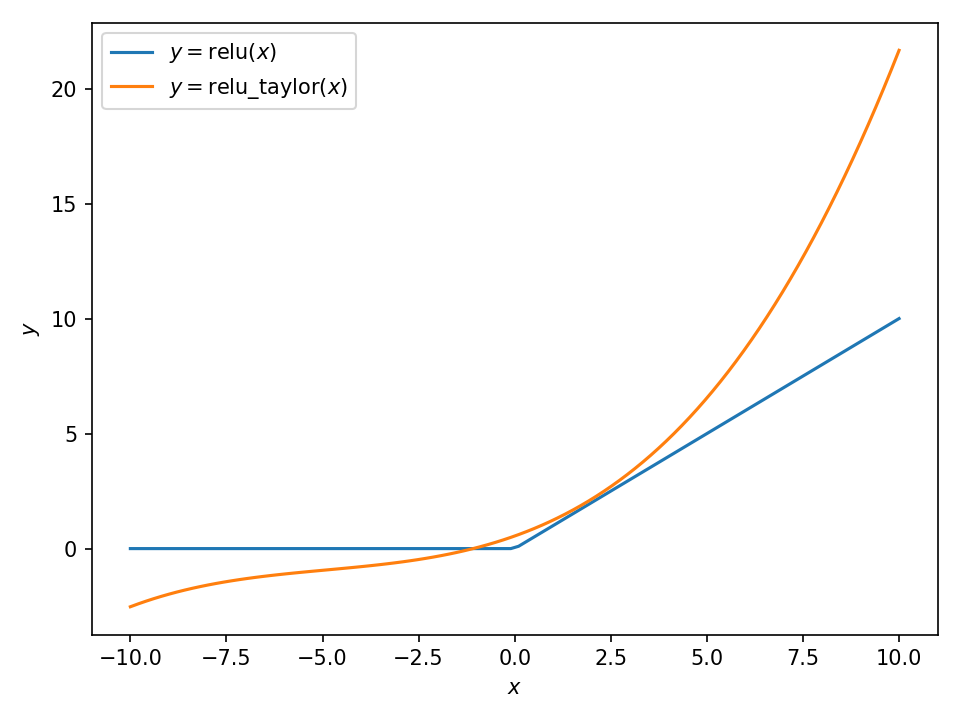
\includegraphics[width=0.8\linewidth]{figures/taylor-relu.png}
  \caption{Comparison of the Relu activation function vs. its Taylor expansion}
\end{figure}

  \chapter{Homomorphic Encryption}
\label{chap:homomorphic-encryption}

\gls{he} makes it possible to operate on data without knowing it.
One can distinguish three flavors of it, Partial-, Somewhat-, Levelled- and \gls{fhe}.

For \Gls{fhe}, there exist a few schemes in use today with existing implementations.
\begin{itemize}
  \item \gls{bfv} scheme for integer arithmetic \parencite{2012-fv-original, 2012-brakerski}.
  \item \gls{bgv} scheme for integer arithmetic \parencite{2012-bgv-original}.
  \item \gls{ckks} scheme for (complex) floating point arithmetic \parencite{2017-ckks-original}.
  \item \gls{fhew} scheme for Boolean circuit evaluation \parencite{2015-fhew-original}.
  \item \gls{tfhe} scheme for Boolean circuit evaluation \parencite{2019-tfhe-original}.
\end{itemize}

We will first introduce the BFV scheme (integer arithmetic) as it represents a fundamental building block behind CKKS.
Due to the inherent applications, this thesis will focus on the CKKS scheme to perform homomorphic operations on (complex-valued) floating point numbers and vectors.

To alleviate upcoming notation, for two tuples $(\cdot, \cdot)$ defined over the same ring, denote their element-wise addition as $(\cdot, \cdot) + (\cdot, \cdot)$, element-wise multiplication by a scalar $u$ as $u \cdot (\cdot, \cdot)$ and element-wise rounding as $\lfloor (\cdot, \cdot) \rceil$.

\section{Homomorphic Encryption using RSA}
In order to illustrate the basic idea behind \Gls{he}, without distancing ourselves too far from the original goal of introducing basic \gls{he} operations used in practice, this short section aims to motivate the definition of ring homomorphisms (cf. \cref{def:ring-homomorphism}) behind a cryptographic background.

With unpadded RSA \parencite{1983-rsa}, some arithmetic can be performed on the ciphertext - looking at the encrypted ciphertext $\mathcal{E}: \Z/q\Z \mapsto \Z/q\Z,\, \mathcal{E}(m) := m^r \mod q$ ($r, q \in \N$) of the message $m_1, m_2 \in \Z/q\Z$ respectively, the following holds:
\begin{align*}
  \mathcal{E}(m_1) \cdot \mathcal{E}(m_2)
   & \equiv (m_1)^r (m_2)^r \mod q            \\
   & \equiv (m_1 m_2)^r \mod q                \\
   & \equiv \mathcal{E}(m_1 \cdot m_2) \mod q
\end{align*}

\gls{rsa} encryption (even supporting an unbounded number of modular multiplications) therefore fulfills the properties of a multiplicative ring homomorphism, which in general terms is defined as follows:

\begin{definition}{Ring Homomorphism}{ring-homomorphism}
  Given two \hyperref[def:ring]{rings} $(R, +, \cdot)$ and $(S, \oplus, \otimes)$, we call a mapping $\varphi: R \rightarrow S$ a ring homomorphism when it satisfies the following conditions:
  $$\forall a, b \in R: \varphi(a + b) = \varphi(a) \oplus \varphi(b) \wedge \varphi(a \cdot b) = \varphi(a) \otimes \varphi(b)$$
\end{definition}

As we can see, the term \glsdesc{he} originates from the ability to perform computations on encrypted data while ensuring the same results are obtained when the same operations are applied to the original data.

\section{Gentry's FHE-Scheme and BGV}
Homomorphic encryption was envisioned by \citeauthor{1978-he-envisioned} as early as the 70's but remained a phantasm for almost three decades and was since referred to as the 'holy grail' of cryptography.
The first fully homomorphic encryption scheme was introduced in Craig \name{Gentry}'s PhD thesis, based on lattice problems \parencite{2009-gentry-fhe-original}.
In earlier schemes, each \gls{he} operation increases noise, making it partially homomorphic instead of fully homomorphic encryption.
\name{Gentry} devised a technique called \textit{bootstrapping} that evaluates the \textit{decryption} circuit homomorphically and thereby resets the noise introduced by previous operations, enabling true fully homomorphic encryption (\gls{fhe}).
Followup schemes improved his blueprint, Gentry's work is clearly a landmark achievement \parencite{2010-first-glimpse-of-fhe}.

\cite{2012-bgv-original} developed a generalisation of \gls{rlwe} that enables interpolation between \gls{lwe} and \gls{rlwe}, allowing for many improvements on earlier schemes, though mainly relying on \cite{2009-gentry-fhe-original}.
The resulting scheme, referred to as \gls{bgv}, allows for integer arithmetic (addition and multiplication on $\Z/q\Z$). It also employs a modulus reduction technique, greatly extending the homomorphic capacity to a broader class of homomorphic circuits.
\cite{seal-4.0} implements the scheme, enabled using \cpp{seal::scheme_type::bgv}.

\pagebreak
\section{The BFV Scheme}
\label{sec:bfv}
This scheme was developed in two separate publications, whose authors initials it is named after, \cite{2012-brakerski} and \cite{2012-fv-original}.
\gls{bfv} is based on \gls{bgv} and they are very similar in their core ideas, one can even convert a BFV ciphertext to an equivalent BGV ciphertext \parencite{2021-he-revisiting}.
In this section, we will focus on a slightly altered implementation introduced in \cite{2014-fv-comparison}.

\subsection{Scheme Definition}
The \gls{bfv} scheme is a tuple of algorithms, introduced in \cref{def:bfv-scheme}.
To summarise the occuring parameters and variables, a brief overview of all used symbols is provided in \cref{tab:bfv-symbols}.

\begin{definition}{The BFV-Scheme}{bfv-scheme}
  Let $R = \Z[X] / \Phi_d(X)$ be a polynomial ring with $\Phi_d(X)$ the $d$\textsuperscript{th} \hyperref[def:cyclotomic-poly]{cyclotomic polynomial}
  ($\rightarrow d \in \N$) for ciphertexts $c \in R \times R$.
  Introduce $R / qR$ the associated quotient ring of the $q$\textsuperscript{th} coset of $R$ with the modulus $q \in \N$.
  Further let $t \in \N$ denote the message modulus with $1<t<q$
  for plain messages $m \in R/tR$ and define $\delta := \lfloor \frac{q}{t} \rfloor$,
  $\delta\inv = \frac{t}{q}$.

  Introduce three bounded discrete probability distributions $\chi_{key}$, $\chi_{enc}$ and $\chi_{error}$ over $R/qR$, one which is only used once for key generation, another used for \cryptop{BFV.Encrypt} and another (usually Gaussian-like) error distribution for manually inserted error terms (confer the \hyperref[def:lwe-search-problem]{LWE-problem}). For BFV, usually $\chi_{key} = \chi_{enc}$.

  For a polynomial $a \in R/qR$, consider the decomposition $a = \sum_{i=0}^{l-1} a_i w^i$ into base $w \in \N$ obtained by $\cryptop{WordDecomp}: R \mapsto R^l, \cryptop{WordDecomp}(a) = ([a_i]_w)_{i=0}^{l-1}$. \\
  Further let $\cryptop{PowersOf}: R \mapsto R^l$ be defined as $\cryptop{PowersOf}(a) = ([a w^i]_q)_{i=0}^{l-1}$.

  Let the parameters $\mathbb{P} = (d, q, t, \chi_{key}, \chi_{error}, w)$ and $l = \lfloor \log_w(q) \rfloor + 1$.
  \vspace{0.2cm}

  \cryptop{BFV.} \\
  \begin{tblr}{Q[l,h]Q[l,h,\textwidth - 3.5cm]}
    \cryptop{ParamGen}$(\lambda)$ & {
        Choose parameters as defined above, given the
        security parameter $\lambda$, such that $1 < t < q$, $w \geq 2$,
        initialize distributions $\chi_{key}$, $\chi_{enc}$ and $\chi_{error}$
        $\quad\rightarrow \mathbb{P}$} \\
    \cryptop{KeyGen}$(\mathbb{P})$ & {
        Generate the secret key $s \leftarrow \chi_{key}$, sample $\vec{\mu} \in (R/qR)^l$
        from $\chi_{error}$ and choose some $\vec{a} \in (R/qR)^l$ uniformly
        at random, compute the relinearisation key
        $\vec{\gamma} = (\cryptop{PowersOf}(s^2) - (\vec{\mu} + \vec{a} \cdot s), \vec{a})$
        and finally output the public key for uniformly random
        $a \in (R/qR)$ and $\mu \leftarrow \chi_{error}$ with $b =-(a \cdot s + \mu)$
        as $\vec{p} = (b, a)$.
        $\quad\rightarrow \vec{p}, s, \vec{\gamma}$} \\
    \cryptop{Encrypt}$(\vec{p}, m)$ & {
        Let $(b,a) = \vec{p}$, $u \leftarrow \chi_{enc}$, $\mu_1, \mu_2 \leftarrow \chi_{error}$,
        then the ciphertext is $\vec{c} = u \cdot \vec{p} + (\delta m + \mu_1, \mu_2) = (\delta m + bu + \mu_1, au + \mu_2)$
        $\quad\rightarrow \vec{c}$} \\
    \cryptop{Decrypt}$(s, \vec{c})$ & {
        Decrypt $\vec{c} = (c_0, c_1)$ as
        $m = \lfloor \delta\inv [c_0 + c_1 s]_t \rceil \in R/tR$
        $\quad\rightarrow m$} \\
    \cryptop{Add}$(\vec{c}_1, \vec{c}_2)$ & {
        Let $(c_0^1, c_1^1) = \vec{c}_1$ and $(c_0^2, c_1^2) = \vec{c}_2$
        then $\vec{c}_3 = (c_0^1 + c_0^2, c_1^1 + c_1^2) = \vec{c}_1 + \vec{c}_2$
        $\quad\rightarrow \vec{c}_3$} \\
    \cryptop{Mult}$(\vec{c}_1, \vec{c}_2)$ & {
        Output $\overline{\vec{c}} = (
          \lfloor \delta\inv c_0^1 c_0^2 \rceil,
          \lfloor \delta\inv(c_0^1 c_1^2 + c_1^1 c_0^2) \rceil,
          \lfloor \delta\inv c_1^1 c_1^2 \rceil
          )$
        $\quad\rightarrow \overline{\vec{c}}$} \\
    \cryptop{ReLin}$(\overline{\vec{c}}, \vec{\gamma})$ & {
        Using the relin key $\vec{\gamma} = (\vec{b}, \vec{a})$,
        relinearize from $\overline{\vec{c}} = (c_0, c_1, c_2)$ as
        $\vec{c} = (c_0 + \cryptop{WordDecomp}(c_2) \cdot \vec{b}, c_1 + \cryptop{WordDecomp}(c_2) \cdot \vec{a})$
        $\quad\rightarrow \vec{c}$} \\
  \end{tblr}

  \parencite{2012-fv-original, 2012-brakerski}
\end{definition}

\begin{table}[H]
  \centering
  \caption[Summary of the parameters and symbols in BFV]{Summary of the parameters and symbols in BFV.}
  \SetTblrInner{rowsep=0pt}
  \begin{tblr}{rll}
    \hline
    \textbf{Symbol} & \textbf{Space} & \textbf{Explanation} \\
    \hline
    $\lambda$ & $\in \R$ & Security parameter \\
    $d$ & $\in \N$ & Index of the cyclotomic polynomial used in $R$ \\
    $q$ & $\in \N$ & Modulus of the ciphertext space $R/qR$ \\
    $t$ & $\in \N$ & Modulus of the plaintext message space $R/tR$ \\
    $\delta$ & $\in \N$ & Ratio between ciphertext and plaintext modulus \\
    $\delta\inv$ & $\in \R$ & Inversion coefficient of the effect of $\delta$ \\
    $w$ & $\in \N$ & Word size used as basis, e.g. $w = 2$ for bits \\
    $l$ & $\in \N$ & Number of words of size $w$ required to encode $q$ \\
    $s$ & $\in R$ & Secret Key \\
    $\vec{p}$ & $\in (R/qR)^2$ & Public Key $(b, a)$ \\
    $\vec{\gamma}$ & $\in [(R/qR)^l]^2$ & Relinearisation Key \\
    $m$ & $\in R/tR$ & Plaintext Message\\
    $\vec{c}$ & $\in (R/qR)^2$ & Ciphertext \\
    $\overline{\vec{c}}$ & $\in (R/qR)^3$ & Slightly larger ciphertext resulting from multiplication \\
  \end{tblr}
  \label{tab:bfv-symbols}
\end{table}

Parameters in $\mathbb{P}$ described above need to be carefully chosen in order to provide for a certain security level $\lambda$ \footnote{for example, using \url{https://github.com/malb/lattice-estimator}}.
Also note that $q$ or $t$ do not need to be prime and could be chosen e.g. as powers of 2.
Encryption requires the public key, decryption the private key as usual in public-key encryption schemes.
The public key depends on the secret key and is chosen in such a way that the corresponding term cancels out when decrypting, as can be seen in \cref{subsec:bfv-verification}.

Homomorphic Addition, by design, works by simple addition of the corresponding ciphertexts.
Multiplication is based on a similar procedure, but tries to prevent an explosion of the scale by dividing through $\delta$ in all three terms.
Otherwise, the original input would be proportional to $\delta^2$ after multiplication, instead of $\delta$ as expected when decrypting.
The \cryptop{BFV.ReLin} operation then takes care of merging the three-term tuple back into a ciphertext made of two polynomials using the relinearisation key $\vec{\gamma}$.

The diagram in \cref{fig:bfv-overview} shows how a typical encryption process works and which ring each object is part of, also compare \cref{tab:bfv-symbols}.

\begin{figure}[H]
  \centering
  \inputtikz{figures/bfv-schematic}
  \caption[Schematic overview of the BFV scheme]{
    Schematic overview of the BFV scheme, adapted from \cite{2020-cryptotree}.
    A plaintext polynomial $m(X)$ is encrypted to the ciphertext $\vec{c} = \cryptop{BFV.Encrypt}(\vec{p}, m)$ using the public key $\vec{p}$, operated on using a combination of \cryptop{BFV.\{Add, Mult, ReLin\}} ciphertext operations and finally decrypted to a new $\tilde{m} = \cryptop{BFV.Decrypt}(s, \tilde{\vec{c}})$ using the secret key $s$.
  }
  \label{fig:bfv-overview}
\end{figure}

\subsection{Verification of the Additive Homomorphism}
\label{subsec:bfv-verification}
\begin{theorem}{BFV encryption is homomorphic with respect to addition}{bfv-enc-is-homomorphic}
  \cryptop{BFV.Encrypt} should encrypt in such a way that the addition algebra can be retained even in the transformed space, showing that we can indeed refer to it as \hyperref[def:ring-homomorphism]{homomorphic} encryption.
\end{theorem}

\begin{proof}
  Starting out with two messages $m, m' \in R/tR$, two polynomials of degree $N-1$ with $N$ coefficients modulo $t$, we check whether addition of two ciphertexts $\vec{c} = \cryptop{BFV.Encrypt}(\vec{p}, m)$ and $\vec{c}' = \cryptop{BFV.Encrypt}(\vec{p}, m')$ indeed decrypts as $m + m'$.

  The client first creates a secret key $s$ and public key $\vec{p} = (b, a)$ with $b = -(as + \tilde{\mu})$ using $\cryptop{BFV.ParamGen}(\lambda)$ and $\cryptop{BFV.KeyGen}(\mathbb{P})$.
  Encrypting $m$ and $m'$ using the public key, we obtain
  $$\vec{c} = (c_0, c_1) = \begin{pmatrix}
      \delta m + b u + \mu_1 \\
      a u + \mu_2
    \end{pmatrix}^T \quad\text{and}\quad \vec{c}' = (c_0', c_1') = \begin{pmatrix}
      \delta m' + b u' + \mu_1' \\
      a u' + \mu_2'
    \end{pmatrix}^T \,.$$
  Evaluating $\overline{\vec{c}} := \cryptop{BFV.Add}(\vec{c}, \vec{c}') = \vec{c} + \vec{c}'$,
  $$\overline{\vec{c}} = \begin{pmatrix}
      \delta (m + m') + b (u + u') + (\mu_1 + \mu_1') \\
      a (u + u') + (\mu_2 + \mu_2')
    \end{pmatrix}^T = \begin{pmatrix}
      \delta \overline{m} + b \overline{u} + \overline{\mu_1} \\
      a \overline{u} + \overline{\mu_2}
    \end{pmatrix}^T$$
  we obtain a ciphertext that hopefully decrypts to the correct sum.
  Indeed,
  \begin{align*}
    \cryptop{BFV.Decrypt}(s, \overline{\vec{c}})
     & = \lfloor \delta\inv [\overline{c_0} + \overline{c_1} s]_t \rceil                                                                                                                                                         \\
     & = \big\lfloor \delta\inv [\delta \overline{m} + b \overline{u} + \overline{\mu_1} + (a \overline{u} + \overline{\mu_2}) s]_t \big\rceil                                                                                   \\
     & = \big\lfloor [(\delta\inv\delta) \overline{m} + \delta\inv b \overline{u} + \delta\inv \overline{\mu_1} + \delta\inv a s \overline{u} + \delta\inv \overline{\mu_2} s]_t \big\rceil                                      \\
     & = \big\lfloor [\overline{m} - \delta\inv (as + \tilde{\mu}) \overline{u} + \delta\inv \overline{\mu_1} + \delta\inv a s \overline{u} + \delta\inv \overline{\mu_2} s]_t \big\rceil                                        \\
     & = \big\lfloor [\overline{m} - \cancel{\delta\inv as \overline{u}} - \delta\inv \tilde{\mu} \overline{u} + \delta\inv \overline{\mu_1} + \cancel{\delta\inv as \overline{u}} + \delta\inv \overline{\mu_2} s]_t \big\rceil \\
     & = \big\lfloor [\overline{m} + \underbrace{\delta\inv (\overline{\mu_1} + \overline{\mu_2} s - \tilde{\mu} \overline{u})}_{:= \epsilon \,, ||\epsilon|| \ll 1}]_t \big\rceil
    \approx \big\lfloor [\overline{m}]_t \big\rceil = \lfloor \overline{m} \rceil \approx \overline{m}
  \end{align*}
  we arrive at the desired result $\overline{m} = m + m'$ after rounding ($\lfloor \cdot \rceil$) the (real) polynomial to a close element in $R/tR$ using one of several round-off algorithms  (cf. \cite{2013-rlwe-toolkit}).
  Of course, the influx of $\epsilon$ is only neglible if all parameters are carefully chosen as described in \cref{def:bfv-scheme} and the error terms are sufficiently small.
  $$t \ll q \Longrightarrow \delta\inv = t/q \ll 1$$ should be given while also ensuring that the spread of the distributions $\chi_{key}$, $\chi_{enc}$ and $\chi_{error}$ is not too large so that $\overline{\mu_{1,2}}, \overline{u}$ and $\tilde{\mu}$ do not lead to a large $\epsilon$ distorting our final result.
\end{proof}

As the public key $\vec{p} = (b, a)$ corresponds to a sample from the RLWE distribution (\cref{corollary:rlwe-dist}), the implied security of the BFV scheme is given by the hardness assumption of LWE (\cref{thm:lwe-hardness}).
An attacker trying to decrypt a ciphertext $\vec{c}$, given only the public key $\vec{p}$, would thereby need to solve the RLWE search problem (\cref{corollary:search-rlwe}) which is known to be hard \parencite{2010-rlwe-original}.

\cite{seal-4.0} implements the scheme, enabled using \cpp{seal::scheme_type::bfv}.

\pagebreak
\section{The CKKS Scheme}
\label{sec:ckks}
The \gls{ckks} scheme allows us to perform approximate arithmetic on floating point numbers.
Essentially, the idea is to extend \gls{bfv} which allows us to operate on polynomials $p \in R/qR$, by an embedding approach that allows us to encode a (complex) floating point number vector $\vec{z} \in \R^n\, (\C^n)$ as an integer polynomial, similar to what is used in \gls{bfv}.
A main contribution of \gls{ckks} is that we have a homomorphic rounding operation which allows to reduce the scaling factors after mulitplication.
The remaining scheme is then extremely similar to \gls{bfv} and even more to \gls{bgv} which it is based on.

Introduce $d, R, R/qR$ as in \cref{def:bfv-scheme} and further define $\mathcal{S} = \R[X] / \Phi_d(X) \subset R$ a similar polynomial ring to $R$, but over the reals instead of the integers.
Let $N = \varphi(d)$ be the degree of the reducing cyclotomic polynomial of $\mathcal{S}$, confer \cref{def:bounded-polynomials}.
For convenience, we usually choose $d$ a power of $2$ and then, by \cref{thm:power-of-2-cyclo-poly}, $N = \varphi(d) = \frac{d}{2}$ which yields very efficiently multipliable polynomials because the homomorphic multiplication operation can be performed using a \gls{dft} and further optimized using the \gls{fft}, which in its unmodified form only accepts power-of-2 vector sizes \parencite{2017-ckks-original}.

\subsection{Encoding and Decoding}
In addition to encryption and decryption, the \gls{ckks} scheme also defines the \cryptop{CKKS.Encode} and \cryptop{CKKS.Decode} operations, extending possible plain inputs from polynomials $m \in R$ (as in BFV) to complex-valued vectors $\vec{z} \in \C^{N/2}$
\footnote{Many implementations of \gls{bfv} provide similar encoding and decoding procedures, extending the original BFV scheme \parencite{2012-fv-original} to facilitate encrypted vector arithmetic.}.
When encoding a vector of $N/2$ elements into a polynomial, a main goal is of course to ensure that addition and multiplication then correspond to elementwise vector addition and multiplication.
Furthermore, these vectors can be rotated (i.e. shifting the elements by an offset) using the \textit{Galois automorphism}.
We will not discuss it in detail here, nevertheless Galois rotations are heavily used in the implementation to facilitate effective matrix multiplications (confer \cref{sec:matmul}).
In total, the encoding and decoding steps consist of three transformations, $\underline{\pi}$, $\underline{\rho}$ and $\underline{\sigma}$.

\begin{definition}{Canonical Embedding $\underline{\sigma}$}{sigma-transform}
  For a real-valued polynomial $p \in \mathcal{S}$, define the canonical embedding of $\mathcal{S}$ in $\C^N$ as a mapping $\underline{\sigma}: \mathcal{S} \mapsto \C^N$ with $$\underline{\sigma}(p) := \big(p(e^{-2\pi i j / N})\big)_{j \in \Z_d^*}$$
  with $\Z_d^* := \{x \in \Z / d\Z \,|\, \gcd(x, d) = 1\}$ the set of all integers smaller than $d$ that do not share a factor $> 1$ with $d$.
  The image of $\underline{\sigma}$ given a set of inputs $R$ shall be denoted as $\underline{\sigma}(R) \subseteq \C^N$.
  Let the inverse of $\underline{\sigma}$ be denoted by $\underline{\sigma}\inv: \C^N \mapsto \mathcal{S}$.
\end{definition}

All elements of $R$ are also elements of $\mathcal{S}$ since $\Z \subset \mathcal{S}$ which results in $\underline{\sigma}(R) \subset \underline{\sigma}(\mathcal{S})$, every plaintext polynomial $m \in R$ can be encoded into $\underline{\sigma}(R)$.
Also note that evaluating a polynomial on the $n$\textsuperscript{th} roots of unity corresponds to performing a \name{Fourier}-Transform.

Define the commutative subring $(\mathbb{H}, +, \cdot)$ of $(\C^N, +, \cdot)$ on the set
$$\mathbb{H} := \{\vec{z} = (z_j)_{j \in \Z_d^*} \in \C^N : z_j = \overline{z_{-j}} \;\forall j \in \Z_d^*\} \subseteq \C^N$$
of all complex-valued vectors $\vec{z}$ where the first half equals the reversed complex-conjugated second half.

\begin{definition}{Natural Projection $\underline{\pi}$}{pi-transform}
  Let $T$ be a mulitplicative subgroup of $\Z_d^*$ with $\Z_d^* / T = \{\pm 1\} = \{1T, -1T\}$, then the natural projection $\underline{\pi}: \mathbb{H} \mapsto \C^{N/2}$ is defined as
  $$\underline{\pi}\big((z_j)_{j \in \Z_M^*}\big) := (z_j)_{j \in T}$$
  Let its inverse be denoted by $\underline{\pi}\inv: \C^{N/2} \mapsto \mathbb{H}$ and consequently defined as
  $$\underline{\pi}\inv\big((z_j)_{j \in T}\big) := \big(\nu(z_j)\big)_{j \in \Z_M^*} \; \mathrm{with} \; \nu(z_j) = \begin{cases}
      z_j            & \text{if } j \in T \\
      \overline{z_j} & \text{otherwise}
    \end{cases}$$
\end{definition}

The natural projection $\underline{\pi}$ simply halves a vector $\vec{z} \in \mathbb{H}$ to all elements where $j \in T$ to only contain its essential information (the first half), since the second half can easily be reconstructed by element-wise conjugation using $\nu$.
The exact structure of $T$ is given by $\Z_d^* / T = \{\pm 1T\}$ with $+1T$ and $-1T$ denoting multiplicative left cosets of $T$, together forming the \hyperref[def:quotient-group]{quotient group} $(\Z_d^* / T, \cdot)$ over multiplication (denoted $\cdot$ instead of $+$ as in the quotient group definition in the previous chapter).

\paragraph{Further studying $T$.}
We first notice that by \name{Lagrange}'s theorem on finite groups, the number of elements in $T$ is exactly $N / 2$ since $$\frac{|\Z_d^*|}{|T|} = |\{\pm 1\}| \Leftrightarrow \frac{N}{|T|} = 2 \Leftrightarrow |T| = \frac{N}{2}$$ leading to $\underline{\pi}(\mathbb{H}) \subseteq \C^{N/2}$.
Rephrased, we seek a $T \subseteq \Z_d^*$ with $1 \in T$ such that we can fully construct $\Z_d^*$ by the union of the cosets $1T$ and $-1T$, i.e. $\Z_d^* = (1T) \cup (-1T)$.
Note that $T$ is not unique, we can find multiple sets $T$ for which the above holds, for instance by brute force computation:

\begin{minted}{python}
  import itertools, math, numpy as np
  d = 16; Zdstar = [z for z in range(d) if math.gcd(d, z) == 1]
  possible_T = [T for T in itertools.combinations(Zdstar, len(Zdstar) // 2)
    if 1 in T and list(np.unique(list(T) + [(-1*t) % d for t in T])) == Zdstar]
\end{minted}

\paragraph{Example.}
Let $d = 16$, then $\Z_d^* = \{1, 3, 5, 7, 9, 11, 13, 15\}$ and $N = |\Z_d^*| = 8$ and by \name{Lagrange}'s theorem, $|T| = 4$.
Since $(T, \cdot)$ forms a normal subgroup under multiplication, we must have that $1 \in T$ and we can identify all possible subgroups $T$ satisfying $\Z_d^* / T = \{\pm 1T\}$ to be one of
\begin{align*}
  \{1, 3, 5, 7\},
  \{1, 3, 5, 9\},
  \{1, 3, 7, 11\},
  \{1, 3, 9, 11\}, \\
  \{1, 5, 7, 13\},
  \{1, 5, 9, 13\},
  \{1, 7, 11, 13\},
  \{1, 9, 11, 13\}
\end{align*}
using the above Python code. An example of an invalid subset $T$ that does cover the whole original set $\Z_d^*$ would be $T = \{1, 7, 9, 15\}$.

For the purposes of \gls{ckks}, we simply choose a global $T$ that is constant for our encoding and decoding procedure and a given $d$.
The inverse natural projection $\underline{\pi}\inv$ then uniquely constructs a vector in $\mathbb{H}$ by filling in elements $\overline{z_j}$ for $j \notin T$ into $\vec{z}$.
For simplicity, we commonly choose $T$ as the 'first half' of $\Z_d^*$ when sorting in an ascending manner as it is always a valid choice
\footnote{
  This can be seen from the coset $-1T$ which exactly equals the 'missing' half in $\Z_d^*$ when the first half is covered by $1T = T = \{1, 3, 5, ..., N-1\}$ since $-1T = \{-1, -3, -5, ..., -(N-1)\} \equiv \{d-1, d-3, d-5, ..., d-N+1\}$ $(\text{mod}\, d)$ when $d$ a power of 2.
  Then, $(1T) \cup (-1T) = \{1, 3, 5, ..., N-1\} \cup \{d-1, d-3, d-5, ..., d-N+1\} = \{1, 3, 5, ..., N-1, N+1, ..., d-5, d-3, d-1\} = \Z_d^*$.
}.

\begin{definition}{Discretisation to an element of $\underline{\sigma}(R)$}{}
  Using one of several round-off algorithms (cf. \cite{2013-rlwe-toolkit}), given an element of $\mathbb{H}$, define a rounding operation $\underline{\rho}\inv: \mathbb{H} \mapsto \underline{\sigma}(R)$ that maps an $\vec{h} \in \mathbb{H}$ to its closest element in $\underline{\sigma}(R) \subset \mathbb{H}$, also denoted as
  $$\underline{\rho}\inv(\vec{h}) := \lfloor \vec{h} \rceil_{\underline{\sigma}(R)}\,.$$
  Further let $\underline{\rho_\delta}\inv(\vec{h}) = \lfloor \delta \cdot \vec{h} \rceil_{\underline{\sigma}(R)}$ denote the same rounding operation but with prior scaling by a scalar factor $\delta$.
  Note that $\underline{\rho}$ is given directly as the identity operation because all elements of its domain are already elements of its image. Similarly, $\underline{\rho_\delta}\inv(\vec{y}) = \delta\inv \cdot \vec{y}$.
\end{definition}

Because it is not essential to understanding the encryption scheme, we will skip over concrete implementations of the rounding procedure $\underline{\rho}\inv$.
For choosing a \textit{close} element $\vec{g} \in \mathbb{H}$, we must first introduce a sense of proximity, in this case done by the $l_\infty$-norm $||\vec{g} - \vec{h}||_\infty$ of the difference between $\vec{h} \in \mathbb{H}$ and $\vec{g}$.

All in all, $m = \cryptop{CKKS.Encode}(\vec{z}),\, \vec{z} \in \C^{N/2}$ applies all inverse transformations $\underline{\pi}\inv$ (first), $\underline{\rho}\inv$ (second) and $\underline{\sigma}\inv$ (third) to an input vector $\vec{z}$ in order to finally arrive at a plaintext polynomial $m \in R/q_L R$ (equally stated as $m \in \Z_{q_L} / (X^N + 1)$ as long as $N$ is a power of 2).
Although $\underline{\sigma}$ is defined over $\mathcal{S}$ instead of $\mathcal{R}$, all elements of $\underline{\sigma}(R)$ can indeed be mapped back to an element in $R$ using $\underline{\sigma}\inv$.
Summarised,
$$\C^{N/2} \xlongrightarrow{\;\underline{\pi}\inv\;} \mathbb{H} \xlongrightarrow{\;\underline{\rho}\inv\;} \sigma(R) \xlongrightarrow{\;\underline{\sigma}\inv\;} R \,.$$
The decoding procedure $\vec{z} = \cryptop{CKKS.Decode}(m),\, m \in R$ does the exact opposite to reobtain the input vector $\vec{z} \in \C^{N/2}$.

It should also be noted that the encoding procedure represents an isometric ring isomorphism (a linear bijection that preserves distance) between its domain and image, as does the decoding procedure.
This reflects in the observation that the plaintext sizes and errors are preserved under the transformations \parencite{2017-ckks-original}.

\pagebreak
\subsection{Scheme Definition}
The \gls{bfv} scheme is a tuple of algorithms, introduced in \cref{def:bfv-scheme}.
To summarise the occuring parameters and variables, a brief overview of all used symbols is provided in \cref{tab:ckks-symbols}.

\begin{definition}{The CKKS Scheme}{ckks-scheme}
  Define $R, R/q_L R$ as in \cref{def:bfv-scheme}.
  Introduce three bounded discrete probability distributions $\chi_{key}$, $\chi_{enc}$ and $\chi_{error}$ over $R/q_L R$.
  \vspace{0.2cm}

  \cryptop{CKKS.} \\
  \begin{tblr}{Q[l,h]Q[l,h,\textwidth - 3.5cm]}
    \cryptop{ParamGen}$(\lambda)$ & {
        Choose parameters as defined above, given the security parameter $\lambda$ and space modulus $q_L$, choose $d \in \N$ a power of $2$, $P, h \in \Z$, $\sigma \in \R$ and initialize distributions $\chi_{key}$, $\chi_{enc}$ and $\chi_{error}$.
        $\quad\rightarrow \mathbb{P}$} \\
    \cryptop{KeyGen}$(\mathbb{P})$ & {
        Sample the secret key $s \leftarrow \chi_{key}$, $a \in R_{q_L}$ uniformly at random, $\mu \leftarrow \chi_{error}$ and obtain the public key $\vec{p} = (b, a)$
        with $b = -a \cdot s + \mu$.
        Sample $a' \in R_{P \cdot q_L}$ uniformly at random, $\mu' \leftarrow \chi_{error}$
        and obtain the evaluation key $\vec{\gamma} = (b', a')$
        with $b' = -a' \cdot s + \mu' + Ps^2$.
        $\quad\rightarrow \vec{p}, s, \vec{\gamma}$} \\
    \cryptop{Encode}$(\vec{z})$ & {For a given input vector $\vec{z}$, output
        $m = (\underline{\sigma}\inv \circ \underline{\rho_\delta}\inv \circ \underline{\pi}\inv)(\vec{z}) = \underline{\sigma}\inv(\lfloor \delta \cdot \underline{\pi}\inv(\vec{z})\rceil_{\underline{\sigma}(R)})$ $\quad\rightarrow m$} \\
    \cryptop{Decode}$(m)$ & {Decode plaintext $m$ as
        $\vec{z} = (\underline{\pi} \circ \underline{\rho_\delta} \circ \underline{\sigma})(m) = (\underline{\pi} \circ \underline{\sigma})(\delta\inv m)$
        $\quad\rightarrow \vec{z}$} \\
    \cryptop{Encrypt}$(\vec{p}, m)$ & {
        Let $(b,a) = \vec{p}$, $u \leftarrow \chi_{enc}$, $\mu_1, \mu_2 \leftarrow \chi_{error}$,
        then the ciphertext is $\vec{c} = u \cdot \vec{p} + (m + \mu_1, \mu_2) = (m + bu + \mu_1, au + \mu_2)$
        $\quad\rightarrow \vec{c}$} \\
    \cryptop{Decrypt}$(s, \vec{c})$ & {
        Decrypt the ciphertext $\vec{c} = (c_0, c_1)$ as $m = \lbrack c_0 + c_1 s\rbrack_{q_L}$
        $\quad\rightarrow m$} \\
    \cryptop{Add}$(\vec{c}_1, \vec{c}_2)$ & {
        Output $\vec{c}_3 = \vec{c}_1 + \vec{c}_2$
        $\quad\rightarrow \vec{c}_3$} \\
    \cryptop{Mult}$(\vec{c}_1, \vec{c}_2)$ & {
        Output $\overline{\vec{c}} = (
          c_0^1 c_0^2,
          c_0^1 c_1^2 + c_1^1 c_0^2,
          c_1^1 c_1^2
          )$
        $\quad\rightarrow \overline{\vec{c}}$} \\
    \cryptop{ReLin}$(\overline{\vec{c}}, \vec{\gamma})$ & {
        Using the evaluation key $\vec{\gamma}$,
        relinearize from $\overline{\vec{c}} = (c_0, c_1, c_2)$ to
        $\vec{c} = (c_0, c_1) + \lfloor P\inv c_2 \vec{\gamma} \rceil$
        $\quad\rightarrow \vec{c}$} \\
    \cryptop{ReScale}$(\vec{c})$ & {
    In order to rescale a ciphertext from level $l_{old}$ to $l_{new}$, multiply by a factor $\frac{q_{l_{new}}}{q_{l_{old}}} \in \Q$ and round to the nearest element of $(R/q_{l_{new}} R) \times (R/q_{l_{new}} R)$:
    $\vec{c}_{new} = \big\lfloor \frac{q_{l_{new}}}{q_{l_{old}}} \vec{c} \big\rceil$ $\quad\rightarrow \vec{c_{new}}$
    } \\
  \end{tblr}

  \parencite{2017-ckks-original}
\end{definition}

For more details on the probability distributions, refer to the original CKKS paper \parencite{2017-ckks-original}, with the following naming relations:
$\chi_{key} = \mathcal{H}WT(h)$ over $\{0,\pm 1\}^N$,
$\chi_{error} = \mathcal{DG}(\sigma^2)$ over $\Z^N$ and
$\chi_{enc} = \mathcal{ZO}(0.5)$ another distribution over $\{0,\pm 1\}^N$.

Encryption, decryption, addition and multiplication work similarly as in \cref{def:bfv-scheme}.
Unlike \gls{bfv} however, \gls{ckks} works with different moduli $q_L$ at each level $L$.
This also casts off the need for up- and downscaling by $\delta$ when multiplying ciphertexts.
The \cryptop{CKKS.ReLin} operation serves the same purpose as in \gls{bfv}, the rescaling operation is new however and takes care of the scale management.
\cryptop{CKKS.ReScale} can be employed whenever we want to work with ciphertexts at different levels, modifying a given ciphertext to the scale of the other enables the other operations to work just as usual.
\Cref{fig:ckks-overview} shows the extended course of action in \gls{ckks} with a preceeding encoding and decoding step.

\begin{table}[H]
  \centering
  \caption[Summary of the parameters and symbols in CKKS]{Summary of the parameters and symbols in CKKS.}
  \SetTblrInner{rowsep=0pt}
  \begin{tblr}{rll}
    \hline
    \textbf{Symbol} & \textbf{Space} & \textbf{Explanation} \\
    \hline
    $\lambda$ & $\in \R$ & Security parameter \\
    $d$ & $\in \N$ & Index of the cyclotomic polynomial used in $R$ \\
    $P$ & $\in \Z$ & Factor used during relinearisation \\
    $h$ & $\in \Z$ & Hamming weight of the secret key (used by $\chi_{key}$) \\
    $\sigma$ & $\in \R$ & Standard deviation of the Gaussian $\chi_{error}$ \\
    $q_L$ & $\in \N$ & Modulus of $R/q_L R$ at level $L$ \\
    $\delta$ & $\in \N$ & Scaling factor used when encoding \\
    $\delta\inv$ & $\in \R$ & Inversion coefficient of the effect of $\delta$ \\
    $s$ & $\in \{0,\pm 1\}^N$ & Secret Key \\
    $\vec{p}$ & $\in (R/q_L R)^2$ & Public Key $(b, a)$ \\
    $\vec{\gamma}$ & $\in (R/(P q_L)R)^2$ & Relinearisation Key \\
    $\vec{z}$ & $\in \C^{N/2}$ & Plain input vector \\
    $m$ & $\in R$ & Plaintext Message \\
    $\vec{c}$ & $\in (R/q_L R)^2$ & Ciphertext Message \\
    $\overline{\vec{c}}$ & $\in (R/q_L R)^3$ & Slightly larger ciphertext from multiplication \\
  \end{tblr}
  \label{tab:ckks-symbols}
\end{table}

\begin{figure}[H]
  \centering
  \inputtikz{figures/ckks-schematic}
  \caption[Schematic overview of the CKKS scheme]{
    Schematic overview of CKKS, adapted from \cite{2020-cryptotree}.
    A plain vector $\vec{z} \in \C^{N/2}$ is encoded to a plaintext polynomial $m = \cryptop{CKKS.Encode}(\vec{z})$, encrypted to the ciphertext $\vec{c} = \cryptop{CKKS.Encrypt}(\vec{p}, m)$ using the public key $\vec{p}$, operated on using a combination of \cryptop{CKKS.\{Add, Mult, ReLin, ReScale\}} ciphertext operations and finally decrypted and decoded to a new $\tilde{\vec{z}} = \cryptop{CKKS.Decode}(\cryptop{CKKS.Decrypt}(s, \tilde{\vec{c}}))$ using the secret key $s$.
  }
  \label{fig:ckks-overview}
\end{figure}

\subsection{Verification of the Additive Homomorphism}
\begin{theorem}{CKKS encryption is homomorphic with respect to addition}{ckks-enc-is-homomorphic}
  \cryptop{CKKS.Encode} and \cryptop{CKKS.Encrypt} should encrypt in such a way that the addition algebra can be retained even in the transformed space, showing that we can indeed refer to it as \hyperref[def:ring-homomorphism]{homomorphic} encryption.
\end{theorem}

\begin{proof}
  Similar to the BFV scheme proof (\cref{thm:bfv-enc-is-homomorphic}), we aim to show that two input vectors $\vec{z}, \vec{z}' \in \C^{N/2}$ can be encoded, encrypted and added - and finally decrypted back to $\overline{\vec{z}} = \vec{z} + \vec{z}'$.

  Due to the extremely high similarity of the BFV and CKKS schemes, they are even identical in their encryption, decryption and adding procedures, the only thing that remains to be shown is the additivity (or even linearity) of \cryptop{CKKS.Encode}.

  % As a first step, the client generates the secret key $s$ and public key $\vec{p} = (b, a)$ with $b = -(as + \overline{\mu})$ using $\cryptop{CKKS.ParamGen}(\lambda)$ and $\cryptop{CKKS.KeyGen}(\mathbb{P})$.
  Encoding $\vec{z}$ and $\vec{z}'$ into $m$ and $m'$, we obtain
  $$m := \cryptop{CKKS.Encode}(\vec{z}) = (\underline{\sigma}\inv \circ \underline{\rho_\delta}\inv \circ \underline{\pi}\inv)(\vec{z})$$
  comprised of three transformations $\underline{\sigma}\inv$, $\underline{\rho_\delta}\inv$ and $\underline{\pi}\inv$ which can be studied separately for their approximate additivity.
  If a function is linear and bijective (turning it into an isomorphism), its inverse will also be linear.
  We will utilize this below by only showing the additivity of $\underline{\sigma}$, $\underline{\rho_\delta}$ and $\underline{\pi}$, assuming their (approximate) bijectivity.
  Especially the bijectivity of $\underline{\sigma}$ is cumbersome to show and for more details we refer the reader to \cite{2017-ckks-original}.

  \begin{itemize}
    \item The canonical embedding $\underline{\sigma}$ evaluates an input polynomial on the $N$\textsuperscript{th} roots of unity $\{\xi_j\}_{j \in \Z_d^*}$.
          For any two polynomials $p_1, p_2 \in \mathcal{S}$, $$\underline{\sigma}(p_1 + p_2) = \big((p_1 + p_2)(\xi_j)\big)_{j \in \Z_d^*} = \big(p_1(\xi_j) + p_2(\xi_j)\big)_{j \in \Z_d^*} = \underline{\sigma}(p_1) + \underline{\sigma}(p_2) \,.$$
    \item The rounding operation $\underline{\rho_\delta}\inv$ is only approximately additive due to its nature \footnote{For an illustrative counterexample of the additivity of rounding, refer to \url{https://math.stackexchange.com/questions/58239/linear-functions-with-rounding}.}.
          For any two vectors $\vec{h_1}, \vec{h_2} \in \mathbb{H}$,
          \begin{align*}
            \underline{\rho_\delta}\inv(\vec{h_1} + \vec{h_2})
             & = \lfloor \delta \cdot (\vec{h_1} + \vec{h_2}) \rceil_{\underline{\sigma}(R)}
            = \lfloor \delta \vec{h_1} + \delta\vec{h_2} \rceil_{\underline{\sigma}(R)}
            \approx \lfloor \delta \vec{h_1} \rceil_{\underline{\sigma}(R)} + \lfloor \delta\vec{h_2} \rceil_{\underline{\sigma}(R)} \\
             & \approx \underline{\rho_\delta}\inv(\vec{h_1}) + \underline{\rho_\delta}\inv(\vec{h_2})\,.
          \end{align*}
          Its inverse $\underline{\rho_\delta}$ is fully additive nevertheless, since it acts as the identity (up to a scalar factor) of the subset $\underline{\sigma}(R)$ back to an element of $\mathbb{H}$.
    \item The natural projection $\underline{\pi}$ halves a vector in $\mathbb{H}$ to an element of $\C^{N/2}$ which is naturally linear.
          Consider any $\vec{h_1}, \vec{h_2} \in \mathbb{H}$, then
          $$\underline{\pi}(\vec{h_1} + \vec{h_2}) = ({h_1}_j + {h_2}_j)_{j \in T} = ({h_1}_j)_{j \in T} + ({h_2}_j)_{j \in T} = \underline{\pi}(\vec{h_1}) + \underline{\pi}(\vec{h_2})\,.$$
  \end{itemize}

  As every step in the full encoding process $\underline{\sigma}\inv \circ \underline{\rho_\delta}\inv \circ \underline{\pi}\inv$ is additive, \cryptop{CKKS.Encode} indeed acts additively.
  \cryptop{CKKS.Decode} on the other hand is only approximately additive due to the rounding operation required in between.

  The rest follows from \cref{thm:bfv-enc-is-homomorphic} as encryption and addition of the BFV scheme are identical.
  All in all for \cryptop{CKKS}, using the secret key $s$ and public key $\vec{p}$,
  $$\cryptop{Decode}(
    \cryptop{Decrypt}(s,
    \cryptop{Add}(
    \cryptop{Encrypt}(\vec{p}, \cryptop{Encode}(\vec{z})),
    \cryptop{Encrypt}(\vec{p}, \cryptop{Encode}(\vec{z}'))
    ))) \approx \vec{z} + \vec{z}' \,.$$
  We can conclude that encoding \textit{and} encryption in CKKS are indeed homomorphic with respect to addition.
\end{proof}

As the public key $\vec{p} = (b, a)$ corresponds to a sample from the RLWE distribution (\cref{corollary:rlwe-dist}), the implied security of the CKKS scheme is given by the hardness assumption of LWE (\cref{thm:lwe-hardness}).
An attacker trying to decrypt a ciphertext $\vec{c}$, given only the public key $\vec{p}$, would thereby need to solve the RLWE search problem (\cref{corollary:search-rlwe}) which is known to be hard \parencite{2010-rlwe-original}.

\cite{seal-4.0} implements the scheme, enabled using \cpp{seal::scheme_type::ckks}.

  \chapter{Implementation}
\label{chap:implementation}

\section{Chosen Software Architecture}
In the given setting, the most accessible frontend is commonly a JavaScript web application.

To still make the classification run as quickly and efficiently as possible, a C++ binary runs
in the backend providing an HTTP API to the frontend application.
In order to allow for more flexibility of the HTTP server, the initial approach was to
pipe requests through a dedicated web application framework with database access
that would allow, for instance, user management next to the basic classification.
However, the resulting communication and computation overhead, even when running with very
efficient protocols such as ZeroMQ, was too high.

Extending the accessibility argument to reproducibility, Docker is a very solid choice \parencite{using-docker-in-science}.
To run the attached demo project, simply execute
\begin{minted}{bash}
  docker-compose build
  docker-compose up
\end{minted}
in the 'code' folder and point your browser to \url{https://localhost}.

\subsection{Docker Multi-Stage Build}
An enterprise-grade, scalable deployment is achieved by means of zero-dependency
Alpine Linux images which contain nothing but compiled binaries and linked libraries.


\section{The MNIST dataset}
The MNIST dataset \parencite{mnist-original} contains X train and Y test images with corresponding labels.
In order to stick to the traditional feedforward technique with data represented
in vector format, therefore it is common to reshape data from $(28, 28)$ images (represented as grayscale values in a matrix)
into a $784$ element vector.

\section{Matrix-Vector Multiplication}
The dot product that is required as part of the neural network evaluation process
needs to be implemented on SEAL ciphertexts as well.

There are multiple methods to achieve a syntactically correct dot product (matrix-vector multiplication)
as described by \textcite{2018-gazelle} for square matrices.

\begin{enumerate}
  \item Naive
  \item Diagonal
  \item Hybrid
  \item Babystep-Giantstep
\end{enumerate}

\begin{figure}
  \centering
  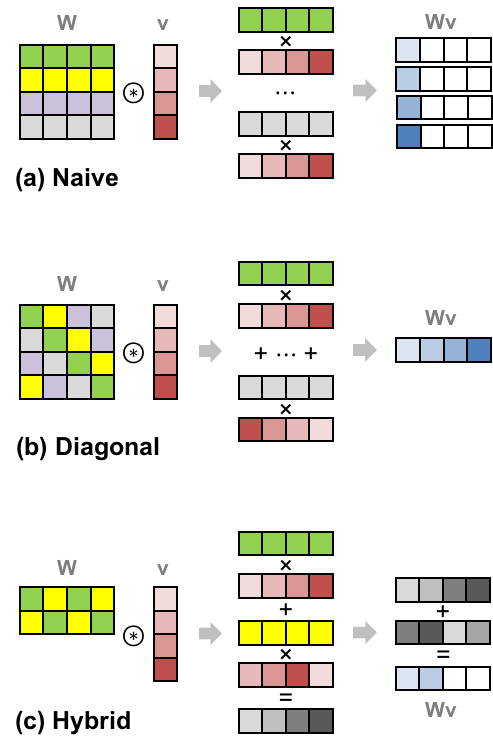
\includegraphics[width=0.4\linewidth]{figures/matrix-vector-multiplication-techniques.png}
  \caption[Image source: \cite{2018-gazelle}]{Different techniques to compute a dot product between a matrix and a vector,
    each having their up- and downsides.}
\end{figure}

\subsection{Adapting to non-square matrices}
The weight matrices in the given classification setting
are by no means square, on the contrary their output dimension tends
to be much lower than the input dimension as the goal is to reduce it from
$28^2 = 784$ to $10$ overall.

However, that also means one cannot directly apply the diagonal method
as described in the proceedings above.
This 'flaw' can be mitigated by a simple zero-padding approach
in order to make the matrix square, filling in zeros until
the lower dimension reaches the higher one.

\subsection{The Naive Method}
Term by term, one can express a matrix-vector product as follows:
$$\{M \vec{x}\}_i = \sum_{j=1}^{t} M_{ij} x_j$$

\subsection{The Diagonal Method}
For the following, define
\newcommand{\rot}{\mathrm{rot}}
\newcommand{\diag}{\mathrm{diag}}
$$\rot_j: \R^t \mapsto \R^t, \; \{\rot_j(\vec{x})\}_i = x_{i + j}$$
$$\diag_j: \R^{t \times t} \mapsto \R^t, \; \{\diag_j(M)\}_i = M_{i, (i+j)}$$
with all indices $i, j \in \Z_t$ member of the cyclic quotient group $\Z_t := \Z / t \Z$ of all integers
modulo $t$, meaning that overflowing indices simply wrap around again starting at index $0$ to simplify notation.
For the sake of compactness, we stick to this notation for the rest of this section.

\subsection{The Hybrid Method}
\subsection{The Babystep-Giantstep Optimization}
Since Galois rotations are the most computationally intensive operations in most cryptographic schemes used
today \parencite{2021-pasta}, they take a large toll on the efficiency.
In order to reduce the number of rotations required, one can make use of the \textit{Babystep-Giantstep}
optimization as described in \cite{2018-faster-helib}, which works as follows:

\begin{theorem}{Babystep-Giantstep Optimization}{bsgs}
  Given a matrix $M \in \R^{t \times t}$ and a vector $\vec{x} \in \R^t$,
  with $t = t_1 \cdot t_2$ split into two BSGS parameters $t_1, t_2 \in \N$ and
  $$\diag'_p(M) = \rot_{-\lfloor p/t_1 \rfloor \cdot t_1}(\diag_p(M))$$,
  one can express a matrix-vector multiplication as follows:
  \begin{equation}
    M \vec{x} = \sum_{k=0}^{t_2-1} \rot_{(kt_1)} \bigg(
    \sum_{j=0}^{t_1-1} \diag'_{(kt_1+j)}(M) \cdot \rot_j(\vec{x})
    \bigg)
  \end{equation}
  where $\cdot$ denotes an element-wise multiplication of two vectors.
\end{theorem}

\begin{proof}
  Starting from the adapted matrix-multiplication expression $P = (P_1, P_2, ..., P_t)^T \in \R^t$,
  we want to show that we indeed end up with an authentic matrix-vector product.
  \begin{align*}
    P = \bigg\{\sum_{k=0}^{t_2-1} \rot_{(kt_1)} \big(
    \sum_{j=0}^{t_1-1} \diag'_{(kt_1+j)}(M) \cdot \rot_j(\vec{x})
    \big)\bigg\}_i = \sum_{k=0}^{t_2-1} \sum_{j=0}^{t_1-1} m'_{kt_1+j,(i+kt_1)} x_{(i+kt_1)+j}
  \end{align*}
  with
  \begin{align*}
    m'_{p,i} = \big\{ diag'_p(M)\big \}_i = \big\{ \rot_{-\lfloor p/t_1 \rfloor \cdot t_1}(\diag_p(M)) \big\}_i
    = M_{i-\lfloor\frac{p}{t_1}\rfloor t_1, i-\lfloor\frac{p}{t_1}\rfloor t_1 + p}
  \end{align*}
  and therefore
  \begin{align*}
    m'_{kt_1+j,i}        & = M_{i-\lfloor\frac{kt_1+j}{t_1}\rfloor t_1, i-\lfloor\frac{kt_1+j}{t_1}\rfloor t_1 + kt_1+j} \\
                         & = M_{i-kt_1-\lfloor\frac{j}{t_1}\rfloor t_1, i-kt_1-\lfloor\frac{j}{t_1}\rfloor t_1 + kt_1+j} \\
                         & = M_{i-kt_1-\lfloor\frac{j}{t_1}\rfloor t_1, i+j-\lfloor\frac{j}{t_1}\rfloor t_1}             \\
    m'_{kt_1+j,(i+kt_1)} & = M_{i+kt_1-kt_1-\lfloor\frac{j}{t_1}\rfloor t_1, i+kt_1+j-\lfloor\frac{j}{t_1}\rfloor t_1}   \\
                         & = M_{i-\lfloor\frac{j}{t_1}\rfloor t_1, i+kt_1+j-\lfloor\frac{j}{t_1}\rfloor t_1}
  \end{align*}
  leading to
  \begin{align*}
    P_i = \sum_{k=0}^{t_2-1} \sum_{j=0}^{t_1-1} m'_{kt_1+j,(i+kt_1)} x_{(i+kt_1)+j}
    = \sum_{k=0}^{t_2-1} \sum_{j=0}^{t_1-1} M_{i-\lfloor\frac{j}{t_1}\rfloor t_1, i+kt_1+j-\lfloor\frac{j}{t_1}\rfloor t_1} x_{(i+kt_1)+j}
  \end{align*}
  . Noticing that the downward rounded fraction $\lfloor\frac{j}{t_1}\rfloor$ vanishes
  in a sum with $j$ running from $0$ to $t_1-1$, we can simplify to
  \begin{align*}
    P_i = \sum_{k=0}^{t_2-1} \sum_{j=0}^{t_1-1} M_{i,i+kt_1+j} x_{i+kt_1+j}
  \end{align*}
  which contains two sums running to $t_1$ and $t_2$ respectively, containing an expression
  of the form $k \cdot t_1 + j$, which allows us to condense the nested sums into one single
  summation expression, as $$\sum_{k=0}^{t_2-1} \sum_{j=0}^{t_1-1} f(kt_1+j) = \sum_{l=0}^{t-1} f(l)$$
  indeed catches every single value $l \in \{0, 1, 2, ..., t=t_1 \cdot t_2\}$ with $l = kt_1+j$. \\
  In summary, we obtain
  \begin{align*}
    P_i & = \sum_{k=0}^{t_2-1} \sum_{j=0}^{t_1-1} M_{i,i+kt_1+j} x_{i+kt_1+j} \\
        & = \sum_{l=0}^{t-1} M_{i,i+l} x_{i+l}
    = \sum_{\nu=0}^{t-1} M_{i,\nu} x_{\nu}                                    \\
        & = \big\{M \vec{x}\big\}_i
  \end{align*}
  which indeed equals the conventional definition of a matrix-vector product.
\end{proof}

Note that the optimized matrix-vector multiplication only requires $t_1 + t_2$ as
we can store the $t_1$ inner rotations of the vector $x$ for the upcoming evaluations.
For larger matrices and vectors (larger $t$), $t_1 + t_2$ are indeed much smaller than
the conventional number of required rotations in the Diagonal or Hybrid method for instance
which was the point of this modification in the first place.

\section{Polynomial Evaluation}
From the implementation perspective, there are three properties to watch out for when
working with SEAL ciphertexts:

\begin{enumerate}
  \item Scale (retrieved using \cpp{x.scale()})
        \begin{quote}
          Scale has nothing to do with noise. "Scale out of bounds" can appear even if noise is extremely low. Although repeated multiplication of a ciphertext by a plaintext will slowly increase the noise, it is not the reason why you see "scale out of bounds".
          "Scale out of bounds" error specifically means that the scale of a ciphertext or plaintext is larger than the product of all elements in coeff\_modulus. If you perform multiplications without rescaling, you can quickly see this error. The more rescaling you perform, the less elements will be left in coeff\_modulus. Even if you managed to have the same scale in a ciphertext after every multiplication and rescale, eventually the coeff\_modulus can be too small to accommodate another multiplication.
        \end{quote}
        % https://github.com/microsoft/SEAL/issues/182#issuecomment-646234787

        Can be adjusted with: \cpp{evaluator.rescale_inplace()}
  \item Encryption Parameters (retrieved using \cpp{x.parms_id()}) \\
        Can be adjusted with: \cpp{evaluator.mod_switch_to_inplace()}
  \item Ciphertext Size (retrieved using \cpp{x.size()}) \\
        Can be adjusted with: \cpp{evaluator.relinearize_inplace()}
\end{enumerate}

\paragraph{Multiplication}
Each time one multiplies two ciphertexts, the scales multiply (logarithmically, they add up, i.e. the bits are added together).
The chain index reduces by 1. The chain index of an encoded ciphertext depends on the coeff moduli.
There must be enough bits remaining to perform the multiplication, namely log2(scale) bits.

\paragraph{Addition}
The scales must be the same, but luckily they will not change.

\section{Transparent Ciphertext}
\begin{quote}
  The problem is that you are subtracting a ciphertext from itself.
  This kind of operation results in a ciphertext that is identically zero;
  this is called a transparent ciphertext. Such a transparent ciphertext
  is not considered to be valid because the ciphertext reveals its underlying plaintext to anyone who sees it,
  even if they don't have the secret key.
  By default SEAL throws an exception when such a situation is encountered to protect you from a problem you may not have noticed.
  If you truly know what you are doing and want to enable the creation of transparent ciphertexts,
  you can configure SEAL [...].
  \parencite{kim-laine-on-transparent-ciphertexts}
\end{quote}

% https://github.com/microsoft/SEAL/issues/276#issuecomment-777073477
'transparent ciphertexts (a.k.a. ciphertexts whose second polynomial is zero) are malformed and do not need the secret key to decrypt'

  \section{Step 5: Results and Accuracy}
\begin{frame}{Chaos everywhere: The Confusion Matrix}
  \centering
  \scalebox{0.64}{\inputtikz{figures/generated/confusion-matrix}}

  \vspace{-0.3cm}
  Plain Accuracy: \SI{97.6}{\percent}, Encrypted Accuracy: \SI{97.3}{\percent}.
\end{frame}

\begin{frame}{Ciphertext Visualisations}
  \begin{figure}[H]
    \centering
    \scalebox{0.9}{\inputtikz{figures/ciphertext-visualisation}}
    % \caption[Visualisation of the plain input images compared to their ciphertext]{Ciphertext Visualisation: The first row corresponds to the images in plain, the second row depicts an encrypted version, namely the reconstructed polynomial coefficients $\{a_k\}$ of the ciphertext polynomial.}
    \label{fig:ciphertext-visualisation}
  \end{figure}
\end{frame}

  \chapter{Conclusion}
\label{chap:conclusion}
\section{Summary}

\inputtikz{figures/venn-diagram}

\section{Outlook}
% describe existing solutions, approaches, current research, etc.
% -> list the papers in library/ folder?
% (include Fabians master thesis about splitting Relin, Galois keys using SPDZ
% to support multiple data providers (clients) and one server, using normal HE algorithms)

\section{Related Works}
Gazelle (inferred ML) as described by \cite{2018-gazelle}.

Random Forests (RF) on HE as described by \cite{2020-cryptotree}.

  \printnoidxglossary[type=acronym]

  \pagebreak
  \thispagestyle{plain}
  \tcblistof[\section*]{def}{Definitions}
  \addcontentsline{toc}{chapter}{List of Definitions and Theorems}
  \tcblistof[\section*]{thm}{Theorems}
  \tcblistof[\section*]{corollary}{Corollaries}
  \tcblistof[\section*]{lemma}{Lemmata}
  \tcblistof[\section*]{remark}{Remarks}

  \printbibliography[heading=bibintoc]
  \listoffigures
  \appendix
\titleformat{\chapter}[block]{\normalfont\LARGE\bfseries}{Appendix \thechapter \;\textendash\;}{0ex}{\vspace{-4cm}}[\vspace{4.5cm}]
\titlespacing{\chapter}{0cm}{0cm}{0cm}

\chapter{Supplemental Proofs}
\label{chap:appendix}

\section{Power-of-2 Cyclotomic Polynomials}
\label{proof:power-of-2-cyclo-poly}
\begin{proof}[Proof of \cref{thm:power-of-2-cyclo-poly}]
  With $k \in \N$ a positive integer, we want to show that
  $$\Phi_{2^k} (x) = x^{2^{k-1}} + 1\,.$$

  A polynomial $p \in \Z[X]$ with $$p(x) = x^n - a$$ of degree $n$ has $n$ roots
  $$\{x_j\} = \{a^\frac{1}{n} e^{2\pi i \frac{j}{n}} \,|\, j \in \N, j \leq n\}$$
  related by a factor $a^\frac{1}{n}$ to the \hyperref[lemma:nth-roots-of-unity]{$n$\textsuperscript{th} roots of unity} given by powers of $\xi = e^{2\pi i \frac{1}{n}}$.

  It is clear from the fundamental theorem of algebra that the polynomial $p$ with roots $\{x_j\}$ can be factorised as
  $$p(x) = \prod_{j=1}^{n} (x - x_j) = \prod_{j=1}^{n} (x - a^\frac{1}{n} e^{2\pi i \frac{j}{n}})\,.$$

  Fixing $a = -1$, we obtain $p(x) = x^n + 1$ with roots given by
  $$x_j = (-1)^\frac{1}{n} e^{2\pi i \frac{j}{n}}
    = (e^{i\pi})^\frac{1}{n} e^{2\pi i \frac{j}{n}}
    = e^{\frac{i\pi (2j + 1)}{n}}$$
  and according factorisation
  $$p(x) = \prod_{j=1}^{n} (x - e^{\frac{i\pi}{n} (2j + 1)})\,.$$

  Further letting $n = 2^{k-1}$ and observing that
  $$\gcd(2^k, l) = \begin{cases}
      1 & \text{if } l \text{ odd}  \\
      2 & \text{if } l \text{ even}
    \end{cases} \quad l, k \in \N$$
  since a number $2^k$ that can only be decomposed into multiples of $2$
  never shares a factor with an odd number, in accordance with \cref{lemma:nth-roots-of-unity}
  we can conclude that the set of all odd roots of unity is exactly the set of all primitive roots (satisfying $\gcd(2^k, l) = 1$).

  Following from above,
  \begin{align*}
    p(x) = \prod_{j=1}^{2^{k-1}} (x - e^{\frac{i\pi}{n} (2j + 1)})
    = \prod_{\stackrel{l=1}{l \text{ odd}}}^{2^k} (x - e^{\frac{i\pi}{n} l})
    = \prod_{\stackrel{l=1}{\xi^l \text{ primitive}}}^{2^k} (x - \xi^l)
    = \Phi_{2^k}(x)
  \end{align*}
  we arrive exactly at the definition of a cyclotomic polynomial (\cref{def:cyclotomic-poly}). \\
  \parencite{power-of-2-cyclo-poly}
\end{proof}

\section{Babystep-Giantstep Multiplication}
\label{proof:bsgs-matmul}
\begin{proof}[Proof of \cref{thm:bsgs}]
  Starting from the adapted \gls{bsgs} matrix-multiplication result $P = (P_1, P_2, ..., P_t)^T \in \R^t$, we want to show that we indeed end up with an authentic matrix-vector product.
  \begin{align*}
    P_i := \bigg\{\sum_{k=0}^{t_2-1} \rot_{(kt_1)} \big(
    \sum_{j=0}^{t_1-1} \diag'_{(kt_1+j)}(M) \cdot \rot_j(\vec{x})
    \big)\bigg\}_i = \sum_{k=0}^{t_2-1} \sum_{j=0}^{t_1-1} m'_{kt_1+j,(i+kt_1)} x_{(i+kt_1)+j}
  \end{align*}
  with
  \begin{align*}
    m'_{p,i} = \big\{ \diag'_p(M)\big \}_i = \big\{ \rot_{-\lfloor p/t_1 \rfloor \cdot t_1}(\diag_p(M)) \big\}_i
    = M_{i-\lfloor\frac{p}{t_1}\rfloor t_1, i-\lfloor\frac{p}{t_1}\rfloor t_1 + p}
  \end{align*}
  and therefore
  \begin{align*}
    m'_{kt_1+j,i}        & = M_{i-\lfloor\frac{kt_1+j}{t_1}\rfloor t_1, i-\lfloor\frac{kt_1+j}{t_1}\rfloor t_1 + kt_1+j} \\
                         & = M_{i-kt_1-\lfloor\frac{j}{t_1}\rfloor t_1, i-kt_1-\lfloor\frac{j}{t_1}\rfloor t_1 + kt_1+j} \\
                         & = M_{i-kt_1-\lfloor\frac{j}{t_1}\rfloor t_1, i+j-\lfloor\frac{j}{t_1}\rfloor t_1}             \\
    m'_{kt_1+j,(i+kt_1)} & = M_{i+kt_1-kt_1-\lfloor\frac{j}{t_1}\rfloor t_1, i+kt_1+j-\lfloor\frac{j}{t_1}\rfloor t_1}   \\
                         & = M_{i-\lfloor\frac{j}{t_1}\rfloor t_1, i+kt_1+j-\lfloor\frac{j}{t_1}\rfloor t_1}
  \end{align*}
  leading to
  \begin{align*}
    P_i = \sum_{k=0}^{t_2-1} \sum_{j=0}^{t_1-1} m'_{kt_1+j,(i+kt_1)} x_{(i+kt_1)+j}
    = \sum_{k=0}^{t_2-1} \sum_{j=0}^{t_1-1} M_{i-\lfloor\frac{j}{t_1}\rfloor t_1, i+kt_1+j-\lfloor\frac{j}{t_1}\rfloor t_1} x_{(i+kt_1)+j} \,.
  \end{align*}
  Noticing that the downward rounded fraction $\lfloor\frac{j}{t_1}\rfloor$ vanishes
  in a sum with $j$ running from $0$ to $t_1-1$, we can simplify to
  \begin{align*}
    P_i = \sum_{k=0}^{t_2-1} \sum_{j=0}^{t_1-1} M_{i,i+kt_1+j} x_{i+kt_1+j}
  \end{align*}
  which contains two sums running to $t_1$ and $t_2$ respectively, containing an expression of the form $k \cdot t_1 + j$, which allows us to condense the nested sums into one single summation expression, as $$\sum_{k=0}^{t_2-1} \sum_{j=0}^{t_1-1} f(kt_1+j) = \sum_{l=0}^{t-1} f(l)$$ indeed catches every single value $l \in \{0, 1, 2, ..., t=t_1 \cdot t_2\}$ with $l = kt_1+j$. \\
  In summary, we obtain
  \begin{align*}
    P_i & = \sum_{k=0}^{t_2-1} \sum_{j=0}^{t_1-1} M_{i,i+kt_1+j} x_{i+kt_1+j} \\
        & = \sum_{l=0}^{t-1} M_{i,i+l} x_{i+l}
    = \sum_{\nu=0}^{t-1} M_{i,\nu} x_{\nu}                                    \\
        & = \big\{M \vec{x}\big\}_i
  \end{align*}
  which indeed equals the conventional definition of a matrix-vector product.
\end{proof}

\end{document}
